\documentclass[a4paper,12pt]{article}
\usepackage[utf8]{inputenc}
\usepackage[spanish]{babel}
\usepackage{tikz}
\usepackage{geometry}
\usepackage{setspace}
\usepackage{titlesec}
%\usepackage{lmodern}
\usepackage{multicol}
\usepackage{fancyhdr}
\usepackage{graphicx}
%\usepackage{helvet}
%\usepackage{mathptmx}
\usepackage{amsmath}       
\usepackage{amssymb}      
\usepackage{adjustbox}     
\usepackage{lastpage}
\usepackage{pgfplots}
\pgfplotsset{compat=1.17}
\usepackage{amsmath}
\usepackage{minted}
\usepackage{wrapfig}

\usepackage{tabularx}
\usepackage{qrcode}
\usepackage{booktabs}
\usepackage{hyperref}
\usepackage{booktabs}
\usepackage{array}
\usepackage{float}
\usepackage{longtable}  

\renewcommand{\arraystretch}{1.4}
\setlength{\tabcolsep}{8pt} 

\setlength{\footskip}{25pt}
%---------------------------python
\usepackage[T1]{fontenc}
\usepackage[utf8]{inputenc}

\usepackage{listings}
\usepackage{xcolor}

\lstdefinestyle{pythonstyle}{
	language=Python,
	basicstyle=\ttfamily\small,
	keywordstyle=\color{blue},
	stringstyle=\color{red},
	commentstyle=\color{gray},
	numbers=left,
	numberstyle=\tiny\color{gray},
	stepnumber=1,
	numbersep=5pt,
	showspaces=false,
	showstringspaces=false,
	breaklines=true,
	frame=single,
	tabsize=4
}



%-------------------------------Consola
\usepackage{listings}
\usepackage{xcolor}

\lstdefinestyle{consola}{
	backgroundcolor=\color{black!5},
	basicstyle=\ttfamily,
	frame=single,
	keywordstyle=\color{blue},
	commentstyle=\color{gray},
	showstringspaces=false
}

%Plano Z y Z^2

\usepackage[utf8]{inputenc}
\usepackage{amsmath, amssymb}
\usepackage{pgfplots}
\pgfplotsset{compat=1.18}
\usepackage{geometry}
\geometry{a4paper, margin=2.5cm}


\geometry{top=2.5cm, bottom=2.5cm, left=2.5cm, right=1.5cm}

% Estilo de página
\pagestyle{fancy}
\fancypagestyle{miestilo}{
	\fancyhf{} % Limpia encabezado y pie
	
	% Encabezado izquierda: logo
	\fancyhead[L]{%
		\vspace{0.1cm}
		\adjustbox{valign=c,scale=0.15}{%
			\begin{tikzpicture}
				\clip (-3,-2.8) rectangle (3,2.8);
				\draw[black,line width=0.8cm] (-2.3,0)--(2.3,0);
				\draw[black,line width=0.8cm] (0,-2.85)--(0,2.85);
				\draw[black,line width=0.87cm] (0,2.8) circle(2);
				\draw[black,line width=0.87cm] (0,-2.8) circle(2);
			\end{tikzpicture}
		}%
	}
	
	% Encabezado centro: título
	\fancyhead[C]{\textbf{Técnicas Digitales 1   
	}}
	
	% Encabezado derecha: TP y año debajo
	\fancyhead[R]{%
		Practico de Laboratorio N°0 \\ 2026
	}
	
	% Línea en el encabezado y pie
	\renewcommand{\headrulewidth}{0.4pt}
	\renewcommand{\footrulewidth}{0.4pt}
	
	% Pie de página derecha: Página X de Y
	\fancyfoot[R]{Página \thepage\ de \pageref{LastPage}}
}


\begin{document}
	
	% --------- PORTADA ---------
	\pagestyle{empty}
	\begin{center}
		\textbf{\LARGE UNIVERSIDAD TECNOLÓGICA NACIONAL}\\[0.2cm]
		\textbf{\Large FACULTAD REGIONAL CÓRDOBA}\\[0.5cm]
		\textbf{\large INGENIERÍA ELECTRÓNICA}\\[1.5cm]
		
		\begin{tikzpicture}
			\clip (-3,-2.8) rectangle (3,2.8);
			\draw[black,line width=0.8cm] (-2.3,0)--(2.3,0);
			\draw[black,line width=0.8cm] (0,-2.85)--(0,2.85);
			\draw[black,line width=0.87cm] (0,2.8) circle(2);
			\draw[black,line width=0.87cm] (0,-2.8) circle(2);
		\end{tikzpicture}
		
		\vspace{1cm}
		\textbf{\huge Técnicas Digitales 1   
		}\\[0.5cm]
		\rule{\textwidth}{0.4pt}\\[0.3cm]
		\textbf{\Huge Practico de Laboratorio N°0}\\[0.3cm]
		{\large MINILAB}\\[0.3cm]
		\rule{\textwidth}{0.4pt}\\[1.5cm]
	\end{center}
	
	\begin{flushleft}
		\begin{tabular}{@{}ll}
			DOCENTES     & : Esp.Ing. Marcelo Casasnovas\\ 
			& \ \  Ing Florencia Belén Molla JTP \\[0.2cm]
			CÁTEDRA      & :  Técnicas Digitales 1   \\[0.2cm]
			CURSO        & : 3R4 \\[0.2cm]
			ALUMNO      & :
			\begin{tabular}[t]{@{}l l}
				Gonza Elías Noel Imanol           & 87669 \\ 
			\end{tabular}
		\end{tabular}
	\end{flushleft}
	
	\vfill
	\begin{center}
		\textbf{CÓRDOBA, ARGENTINA}\\
		\textbf{2026}
	\end{center}
	\pagestyle{empty}
	% --------- CAMBIO DE ESTILO ---------
	\newpage
	\pagenumbering{arabic}
	\pagestyle{miestilo}
	% --------- CONTENIDO ---------
	\tableofcontents
	\newpage
	
	
	\section*{Introducción}
	\addcontentsline{toc}{section}{Introducción}
	
	El presente informe documenta el diseño y la implementación de un Mini-Lab portátil, desarrollado como herramienta de soporte para la asignatura Técnicas Digitales I. El dispositivo constituye una plataforma de experimentación integral que permite la validación de circuitos integrados lógicos y la simulación de diversos sistemas digitales mediante hardware dedicado.
	
	El proyecto se estructura sobre tres pilares fundamentales: una etapa de regulación de tensión para asegurar una alimentación estable, un generador de señal de reloj (oscilador) basado en el temporizador NE555, un bloque conversor de niveles para la adaptación de señales y una interfaz de entradas/salidas lógicas para la interacción con el usuario. La ejecución de este prototipo abarca desde la captura esquemática en entorno CAD hasta la manufactura de la placa de circuito impreso (PCB) mediante métodos químicos, permitiendo la integración de conceptos teóricos en una solución física funcional.
	\newpage
	
	
	\section*{Fundamento Teórico}
	\addcontentsline{toc}{section}{Fundamento Teórico}
	El \textbf{Mini-Lab} se estructura en torno a tres subsistemas fundamentales que permiten la experimentación con señales digitales y analógicas básicas:
	
	\begin{itemize}
		\item \textbf{Conversores Digitales:} Utiliza el circuito integrado \textbf{CD4049}, el cual provee seis buffers/inversores (NOT). Su función principal es transformar las entradas lógicas en salidas compatibles con niveles TTL de hasta 5\,V.
		\item \textbf{Fuente de Alimentación:} El sistema incorpora un regulador de tensión \textbf{LM7805} para suministrar 5\,V estables. El diseño permite versatilidad en la entrada, admitiendo una batería de 9\,V CC o una fuente conmutada.
		\item \textbf{Generador de Onda Cuadrada (Oscilador):} Basado en el \textbf{NE555} configurado en modo astable. Esta etapa genera una señal periódica cuya frecuencia es ajustable mediante un potenciómetro.
	\end{itemize}
	
	\section*{Lista de Materiales y Componentes}
	\addcontentsline{toc}{section}{Lista de Materiales y Componentes}
	A continuación, se detallan los componentes necesarios para el Minilab.
	
	\begin{table}[H]
		\centering
		\begin{tabular}{@{}llc p{4cm}@{}}
			\toprule
			\textbf{Categoría} & \textbf{Componente / Valor} & \textbf{Cant.} & \textbf{Observaciones} \\
			\midrule
			Semiconductores & CI CD4049 (Inversor Hex) & 1 & Buffer de salida \\
			& CI LM7805 & 1 & Regulador +5V \\
			& Diodo 1N4007 & 1 &  \\
			& CI NE555 & 1 & Oscilador (Opcional) \\
			& LEDs (Varios colores) & 8 & Indicadores de estado \\
			\midrule
			Pasivos & Resistencia 1 k$\Omega$ & 7 & \\
			& Resistencia 10 k$\Omega$ & 4 & \\
			& Resistencia 470 $\Omega$ & 6 & Limitadoras para LEDs \\
			& Potenciómetro 5 k$\Omega$ & 1 & Ajuste de frecuencia \\
			& Cap. Electrolítico 470 $\mu$F & 2 & Filtro de fuente \\
			& Cap. Cerámico 0.1 $\mu$F & 6 & Desacople \\
			\midrule
			Electromecánicos & Llave / Interruptor & 6 & Control de entradas \\
			& Llave Doble Inversora & 1 & Selección de modo \\
			\midrule
			Hardware & Protoboard o Placa de cobre doble faz & 1 & Montaje final \\
			& Conector de Batería 9V / USB & 1 & Alimentación dual \\
			& Conector USB-C & 1 & Alimentación dual \\
			\bottomrule
		\end{tabular}
		\caption{Listado de componentes para el Mini-Lab.}
	\end{table}
	\newpage
	
	
\section*{Diagramas Técnicos y Datasheets}
\addcontentsline{toc}{section}{Diagramas Técnicos y Datasheets}

% --- CD4049 ---
\begin{figure}[H]
	\centering
	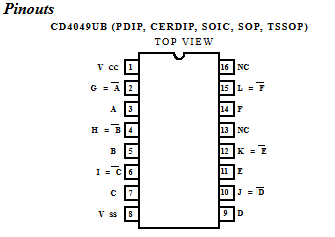
\includegraphics[width=0.45\textwidth]{4049.png}
	\caption{Pinout del Inversor Hexagonal CD4049.}
	\footnotesize \textbf{Datasheet:} \url{https://www.alldatasheet.com/html-pdf/26882/TI/CD4049/20/1/CD4049.html}
\end{figure}

% --- LM7805 ---
\begin{figure}[H]
	\centering
	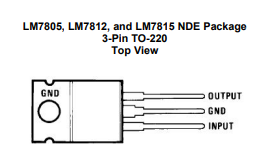
\includegraphics[width=0.3\textwidth]{7805.png} 
	\caption{Conexiones del Regulador LM7805.}
	\footnotesize \textbf{Datasheet:} \url{https://www.alldatasheet.com/html-pdf/82833/FAIRCHILD/LM7805/405/1/LM7805.html}
\end{figure}

% --- NE555 ---
\begin{figure}[H]
	\centering
	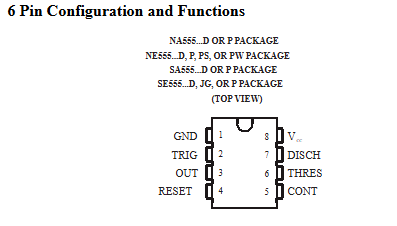
\includegraphics[width=0.6\textwidth]{555.png}
	\caption{Diagrama de pines del Temporizador NE555.}
	\footnotesize \textbf{Datasheet:} \url{https://www.ti.com/lit/ds/symlink/ne555.pdf}
\end{figure}

\begin{figure}[H]
	\centering
	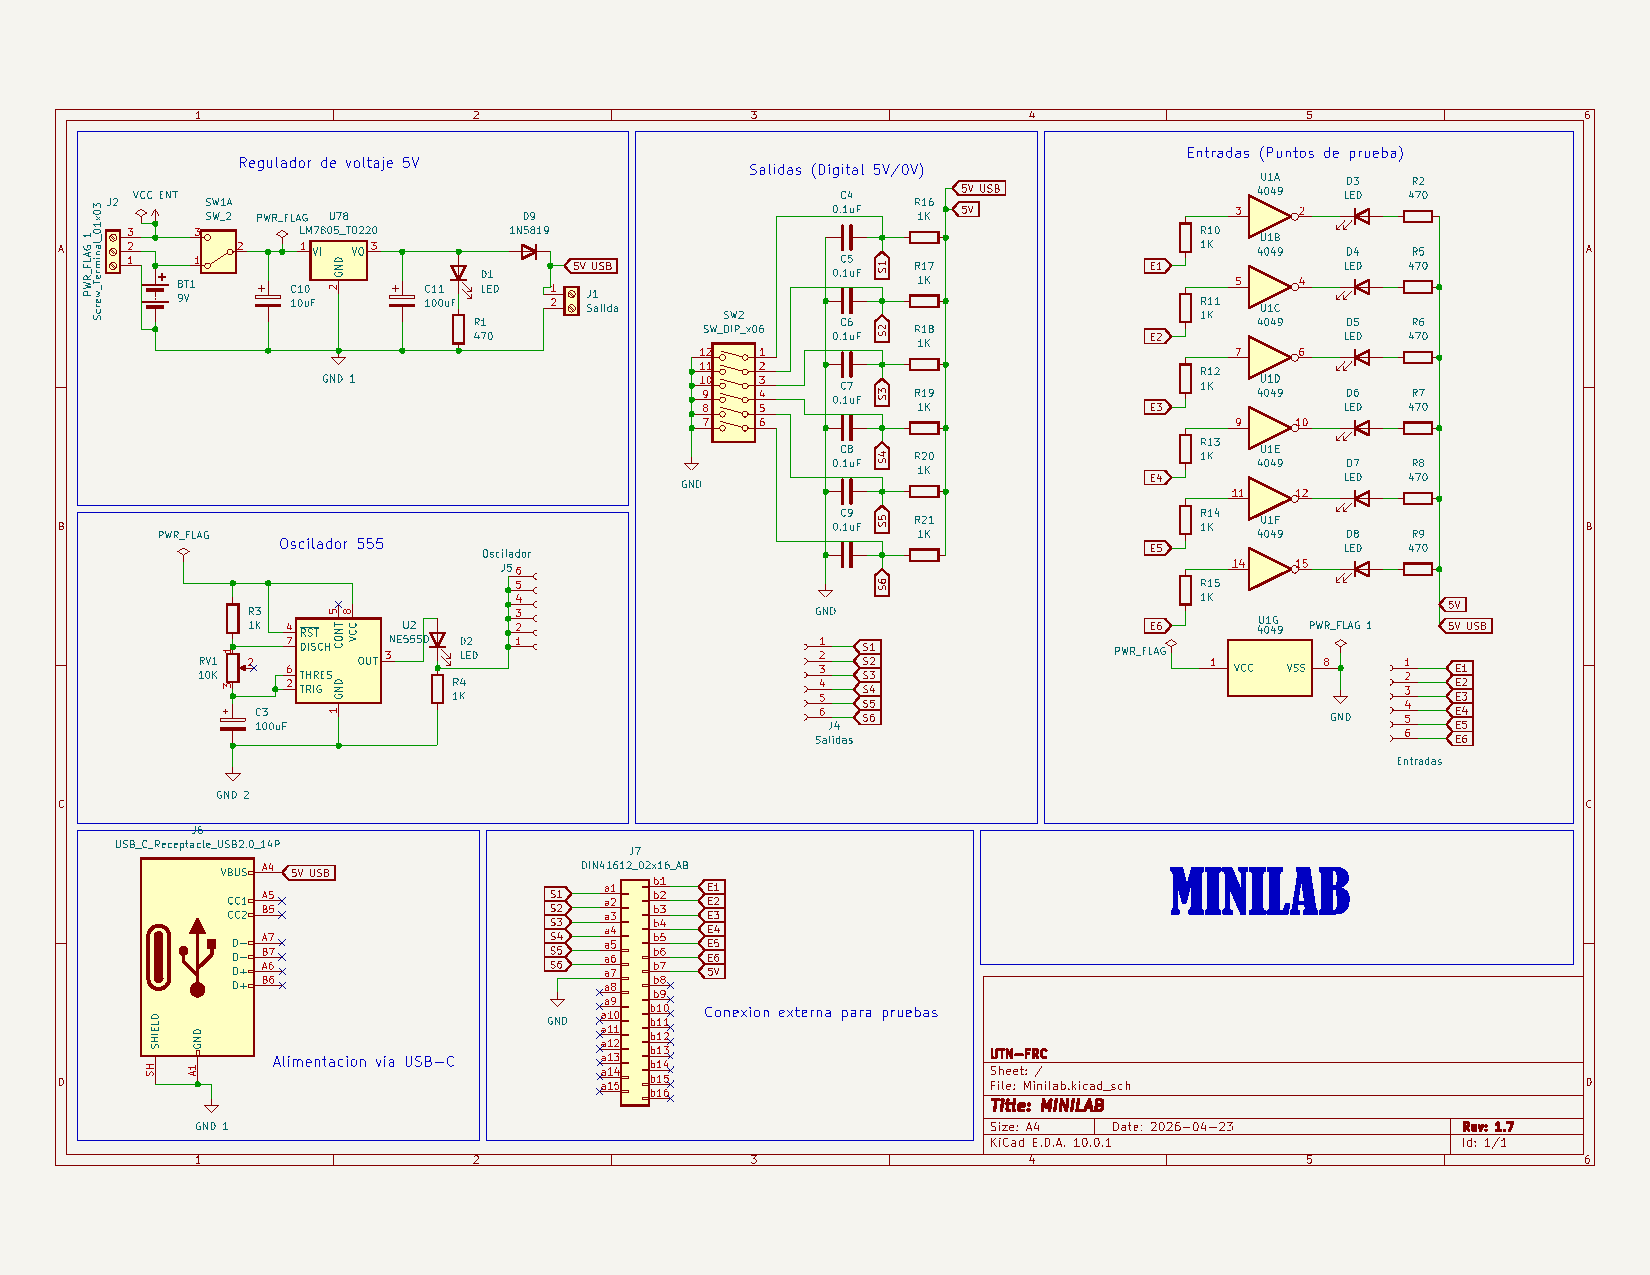
\includegraphics[page=1, width=1.4\textwidth, angle=90]{minilab a.pdf}
	\caption{Diagrama de Kicad del Minilab}
\end{figure}

\begin{figure}[H]
	\centering

	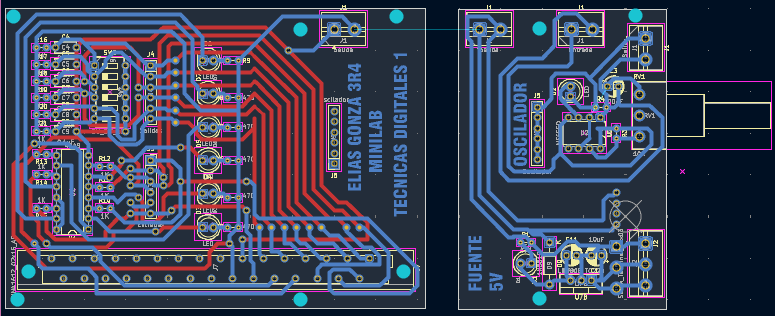
\includegraphics[width=0.8\textwidth]{placa.png} 
	\caption{Vista del diseño de pistas y serigrafía en KiCad.}
	\label{fig:pcb_kicad}
\end{figure}



\section*{Proceso de Fabricación de la Placa (PCB)}
\addcontentsline{toc}{section}{Proceso de Fabricación de la Placa (PCB)}

El proceso de fabricación del \textbf{Mini-Lab} se llevó a cabo mediante el método de transferencia térmica y atacado químico. A continuación, se detallan las etapas realizadas:





\subsection*{Pasos de Ejecución}
\addcontentsline{toc}{subsection}{Pasos de Ejecución}

\begin{enumerate}
	\item \textbf{Impresión:} Se imprimió el diseño en espejo utilizando una impresora láser sobre papel fotográfico (papel ilustración).
	
	\begin{figure}[H]
		\centering
		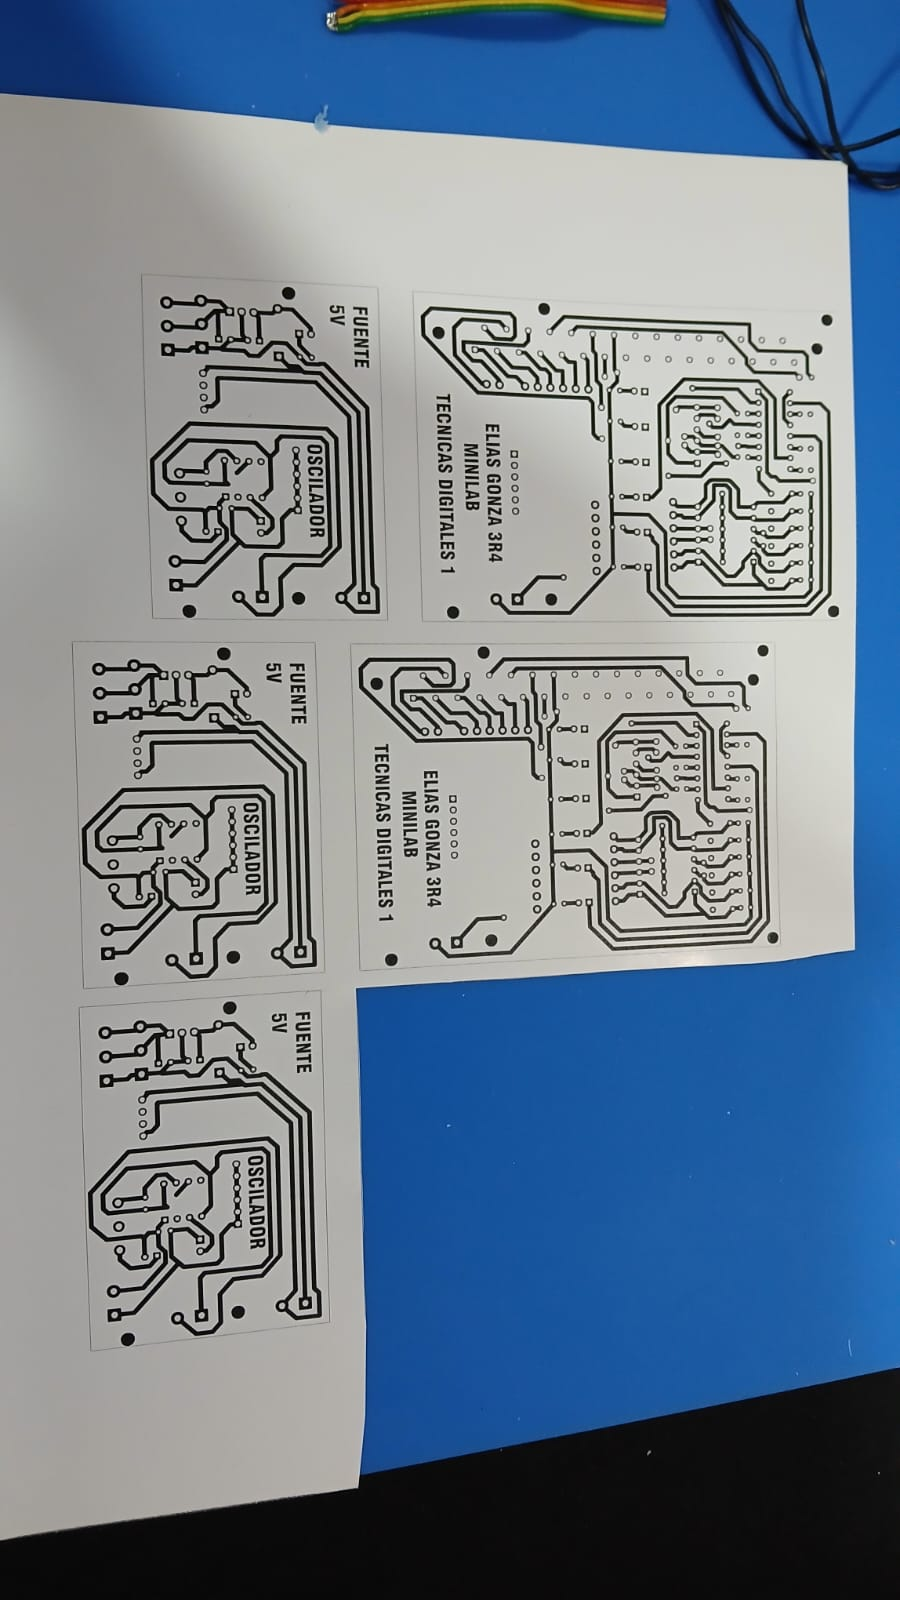
\includegraphics[width=0.4\textwidth, angle=90]{Impresion.jpeg} 
		\caption{Impresion}
	\end{figure}
	

	
	\item \textbf{Transferencia Térmica:} Se limpió la placa de cobre virgen con alcohol isopropílico. Luego, se aplicó calor con una plancha sobre el papel durante aproximadamente 5 minutos para transferir el tóner al cobre.
	
	\begin{figure}[H]
		\centering
		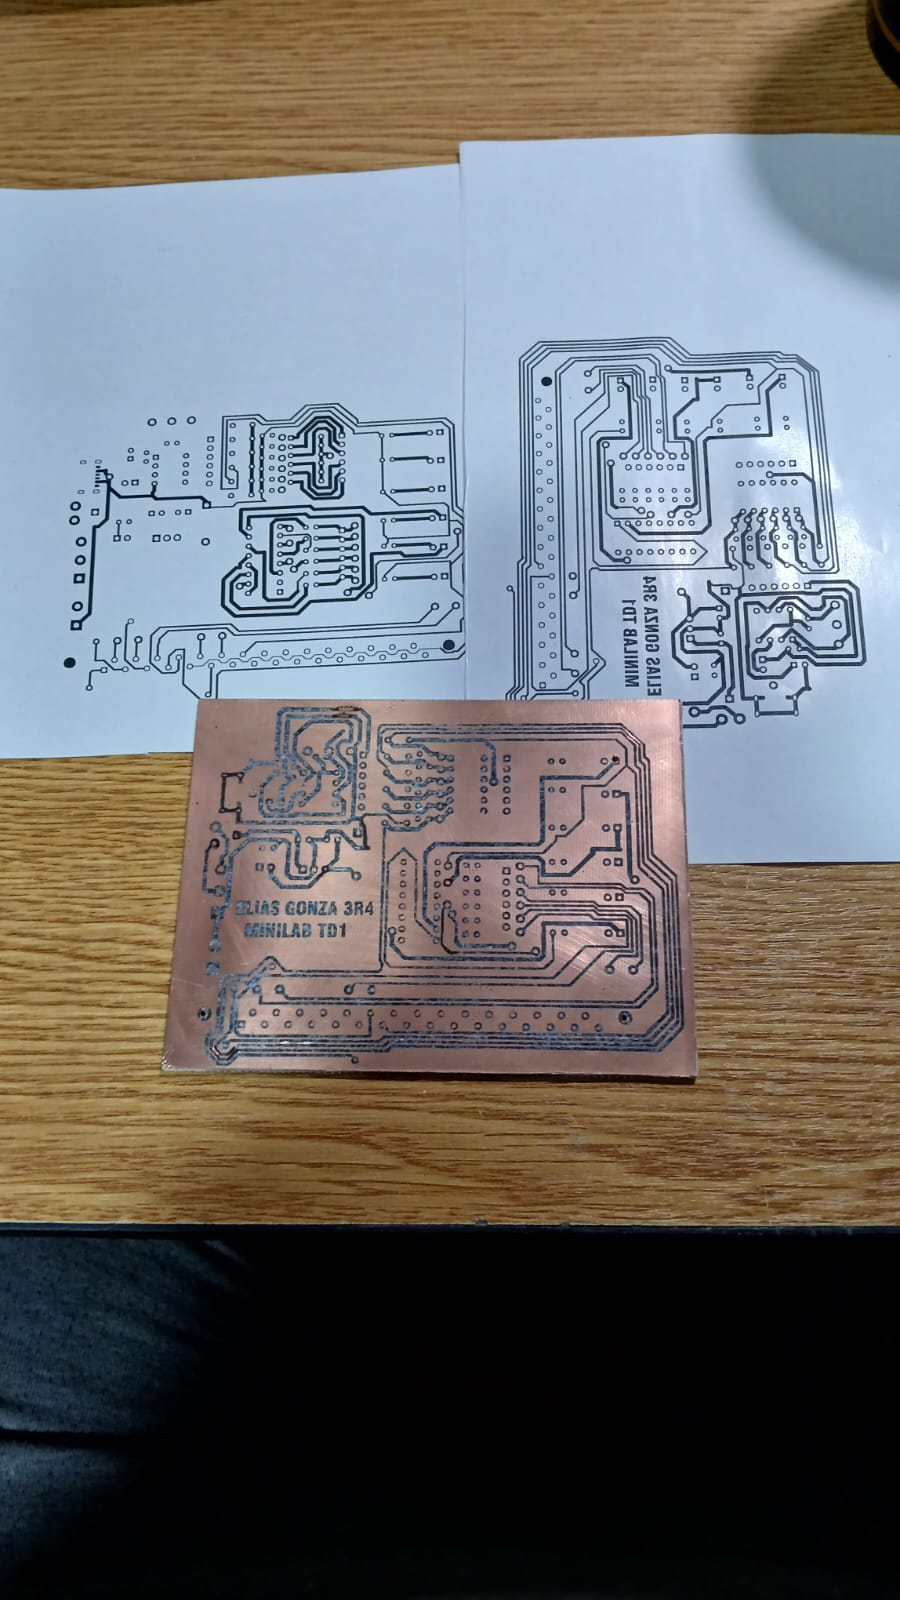
\includegraphics[width=0.4\textwidth, angle=90]{transferencia.jpeg} 
		\caption{Transferencia térmica }
	\end{figure}
	
	
	
	
	\item \textbf{Atacado Químico:} Se sumergió la placa en una solución de cloruro férrico. En esta etapa, el ácido elimina el cobre sobrante, dejando únicamente las pistas protegidas por el tóner.
\end{enumerate}

\begin{figure}[H]
	\centering
	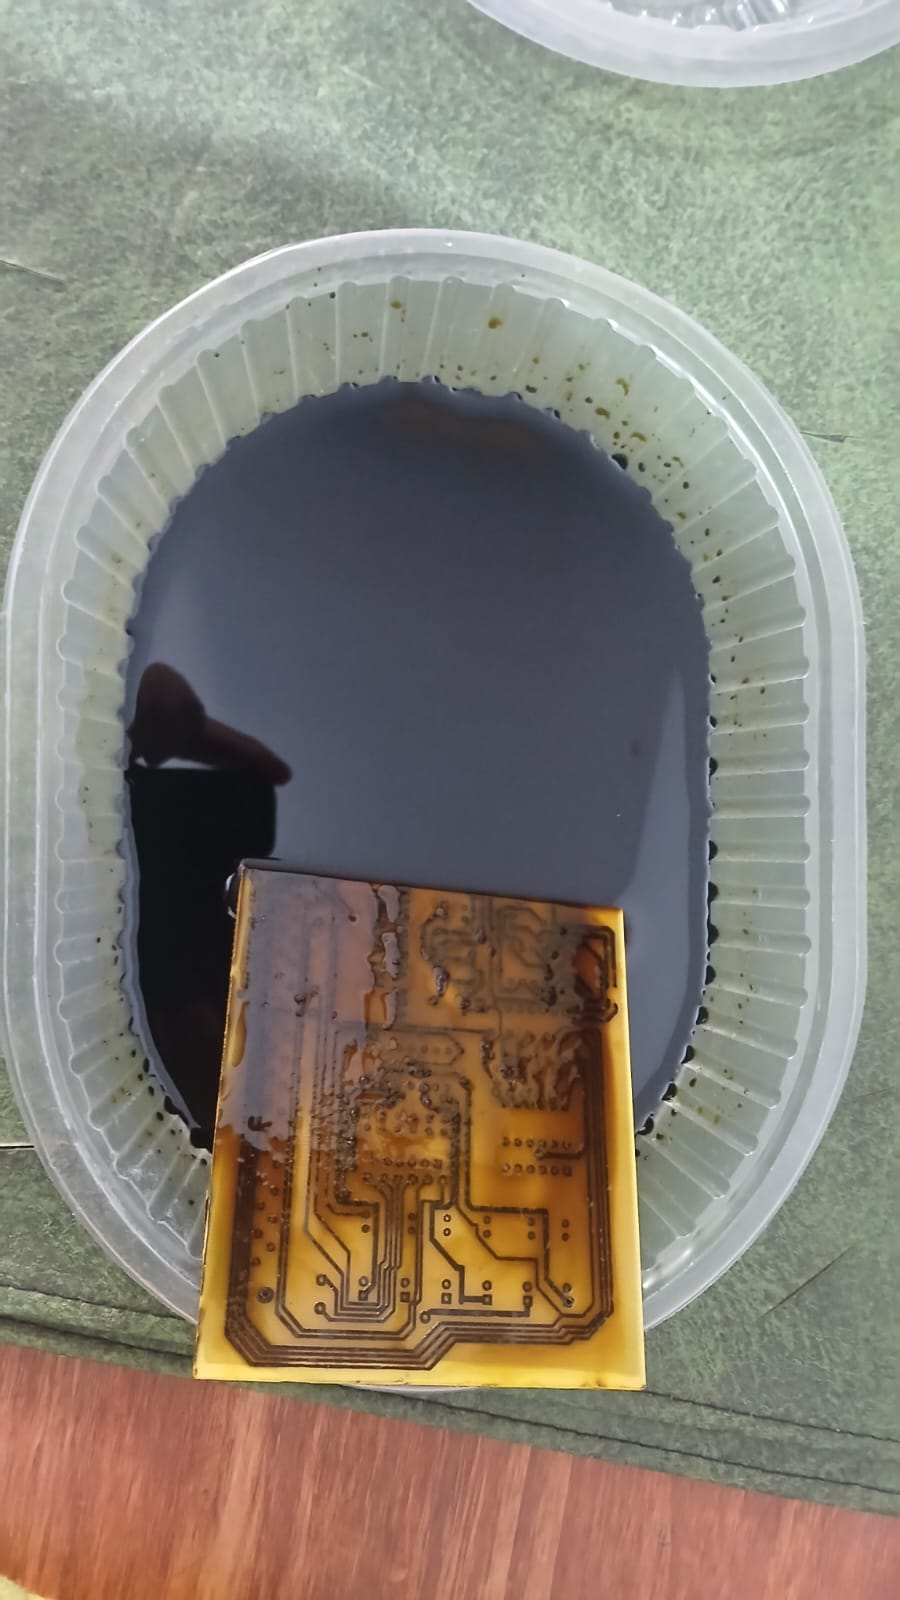
\includegraphics[width=0.4\textwidth,angle=90]{quimico.jpeg} 
	\caption{Grabado químico}
\end{figure}

\subsection*{Finalización y Soldadura}
\addcontentsline{toc}{subsection}{Finalización y Soldadura}
Una vez limpia la placa, se procedió a la perforación con mechas de 1,5 mm y 2 mm. Finalmente, se soldaron los componentes siguiendo el diagrama del minilab.

\begin{figure}[H]
	\centering
	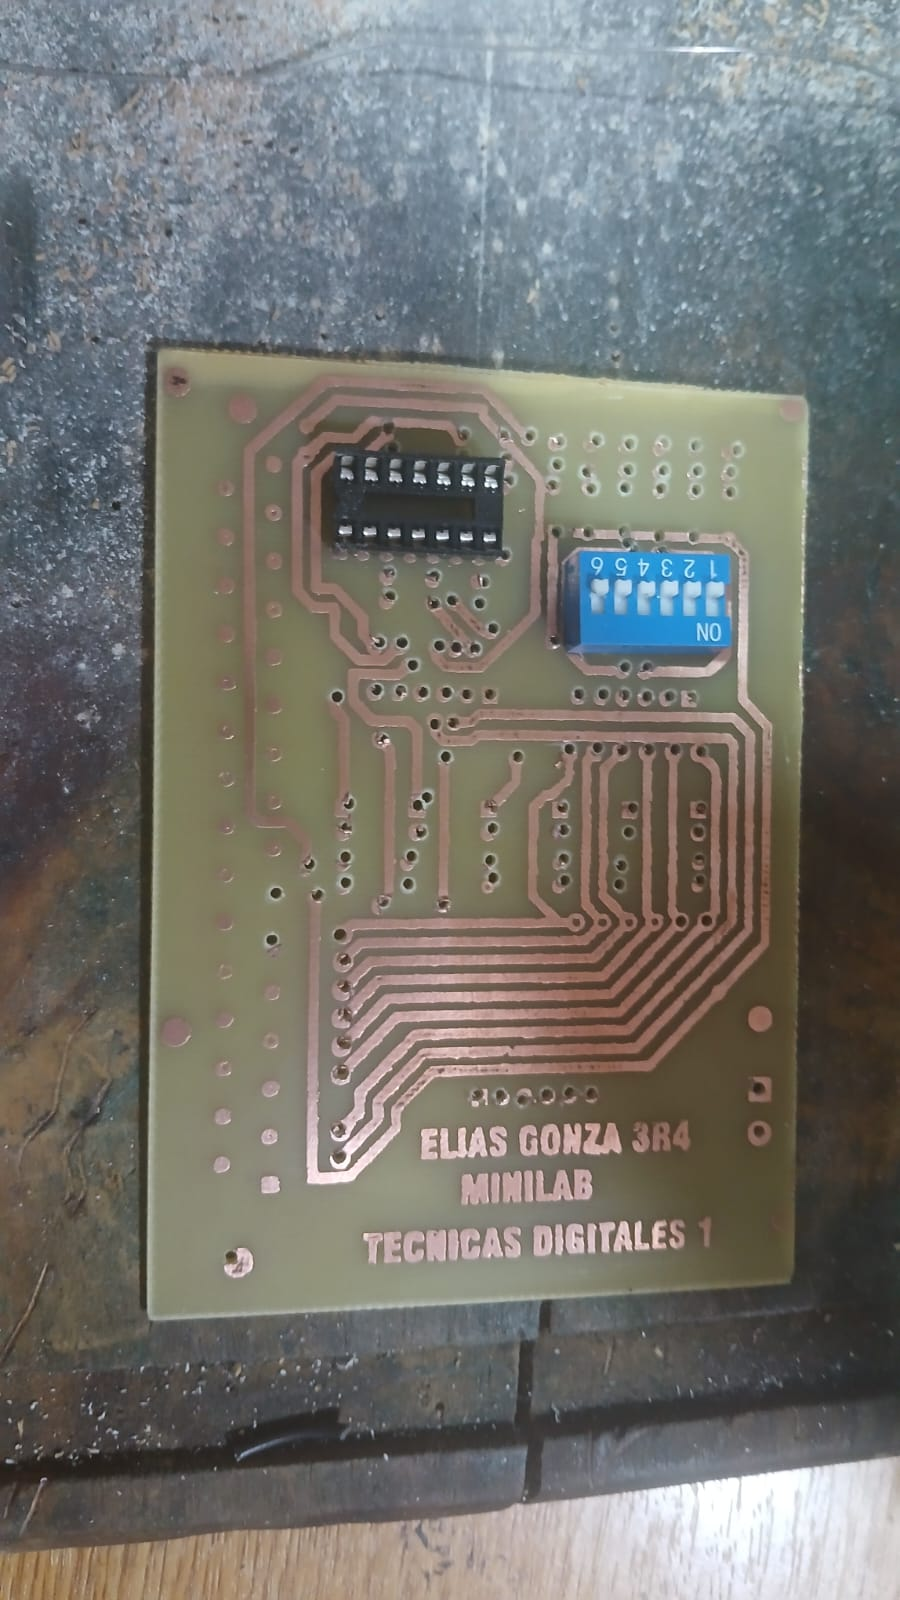
\includegraphics[width=0.4\textwidth,angle=90]{terminado1.jpeg} 
	\caption{Vista de la placa Mini-Lab con las perforaciones.}
\end{figure}

\begin{figure}[H]
	\centering
	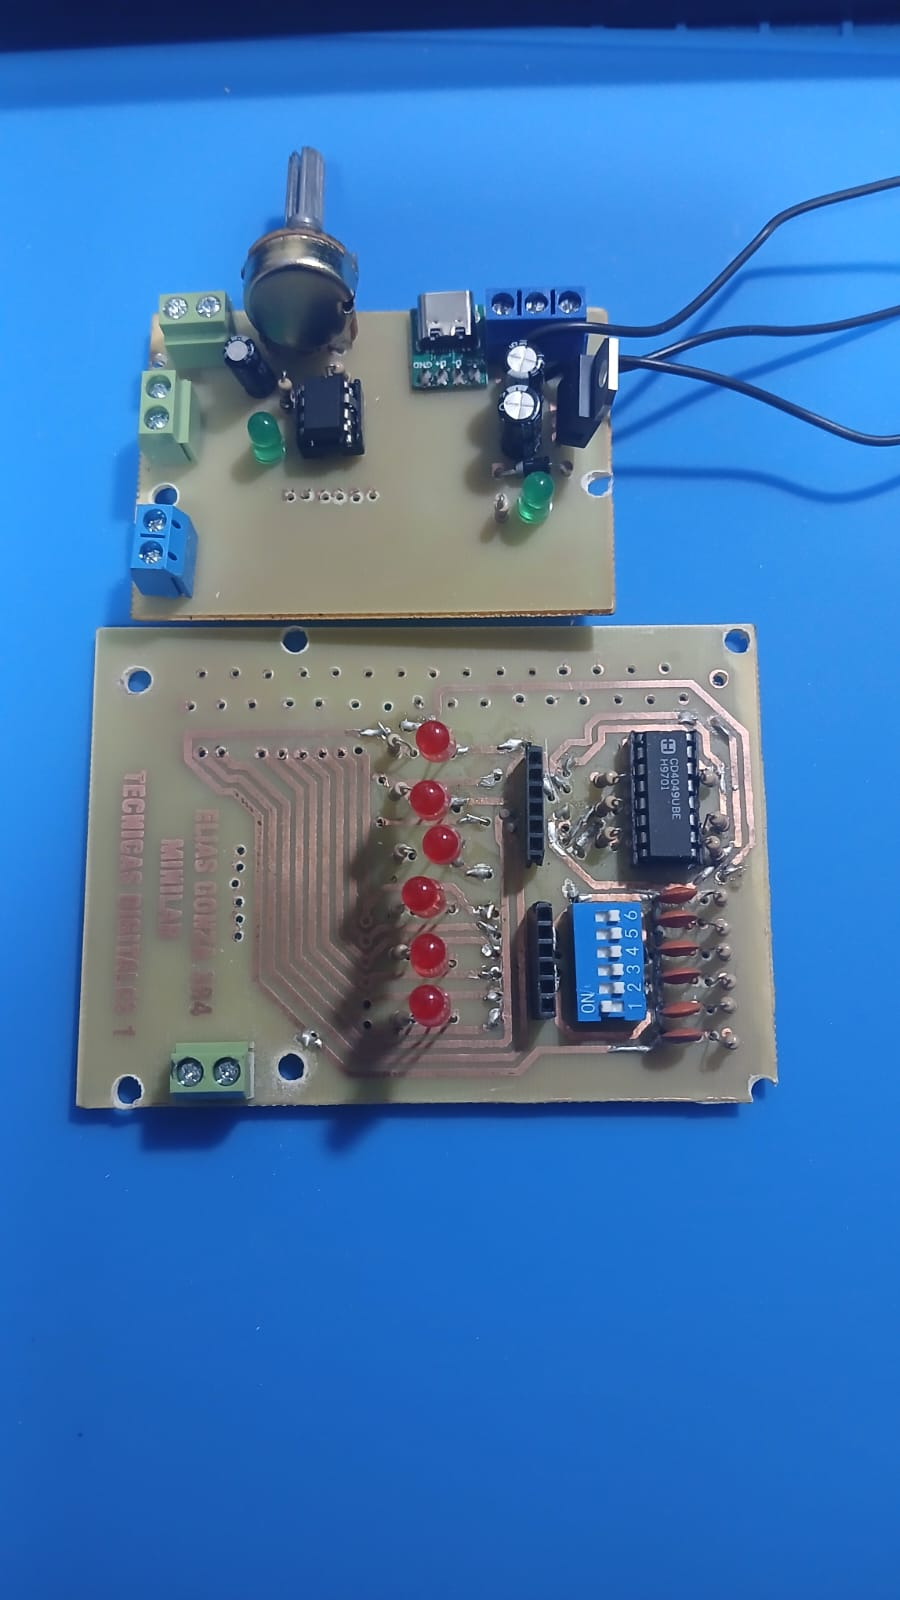
\includegraphics[width=0.4\textwidth,angle=90]{terminado2.jpeg} 
	\caption{Vista de la placa Mini-Lab con los componentes soldados.}
\end{figure}

\begin{figure}[H]
	\centering
	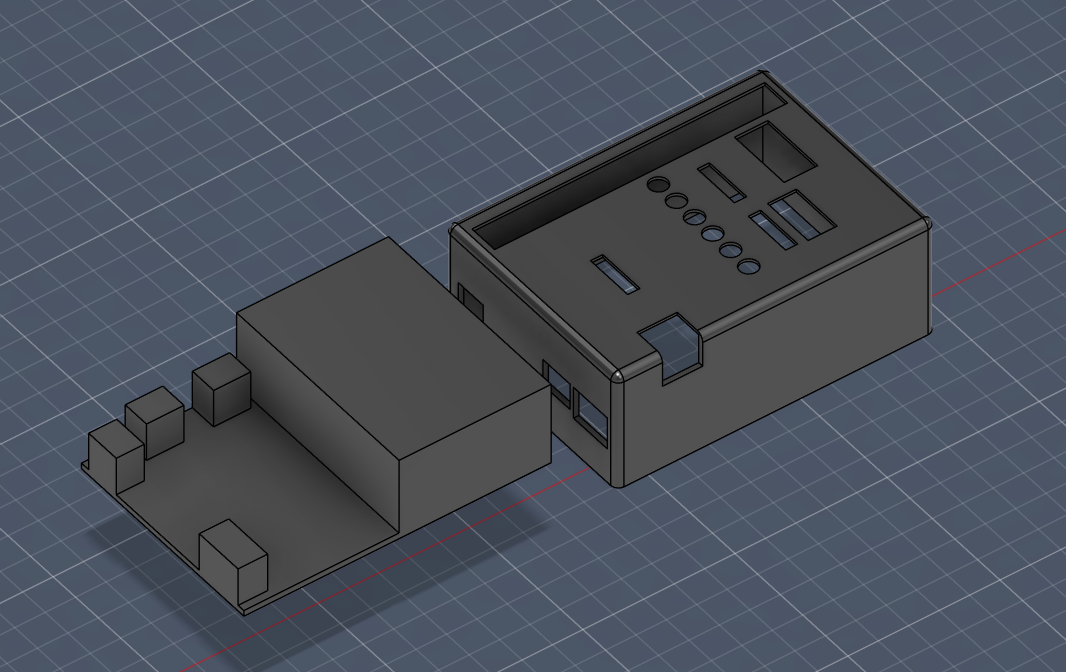
\includegraphics[width=0.6\textwidth]{gabinete.png} 
	\caption{Diseño del gabinete.}
\end{figure}

\begin{figure}[H]
	\centering
	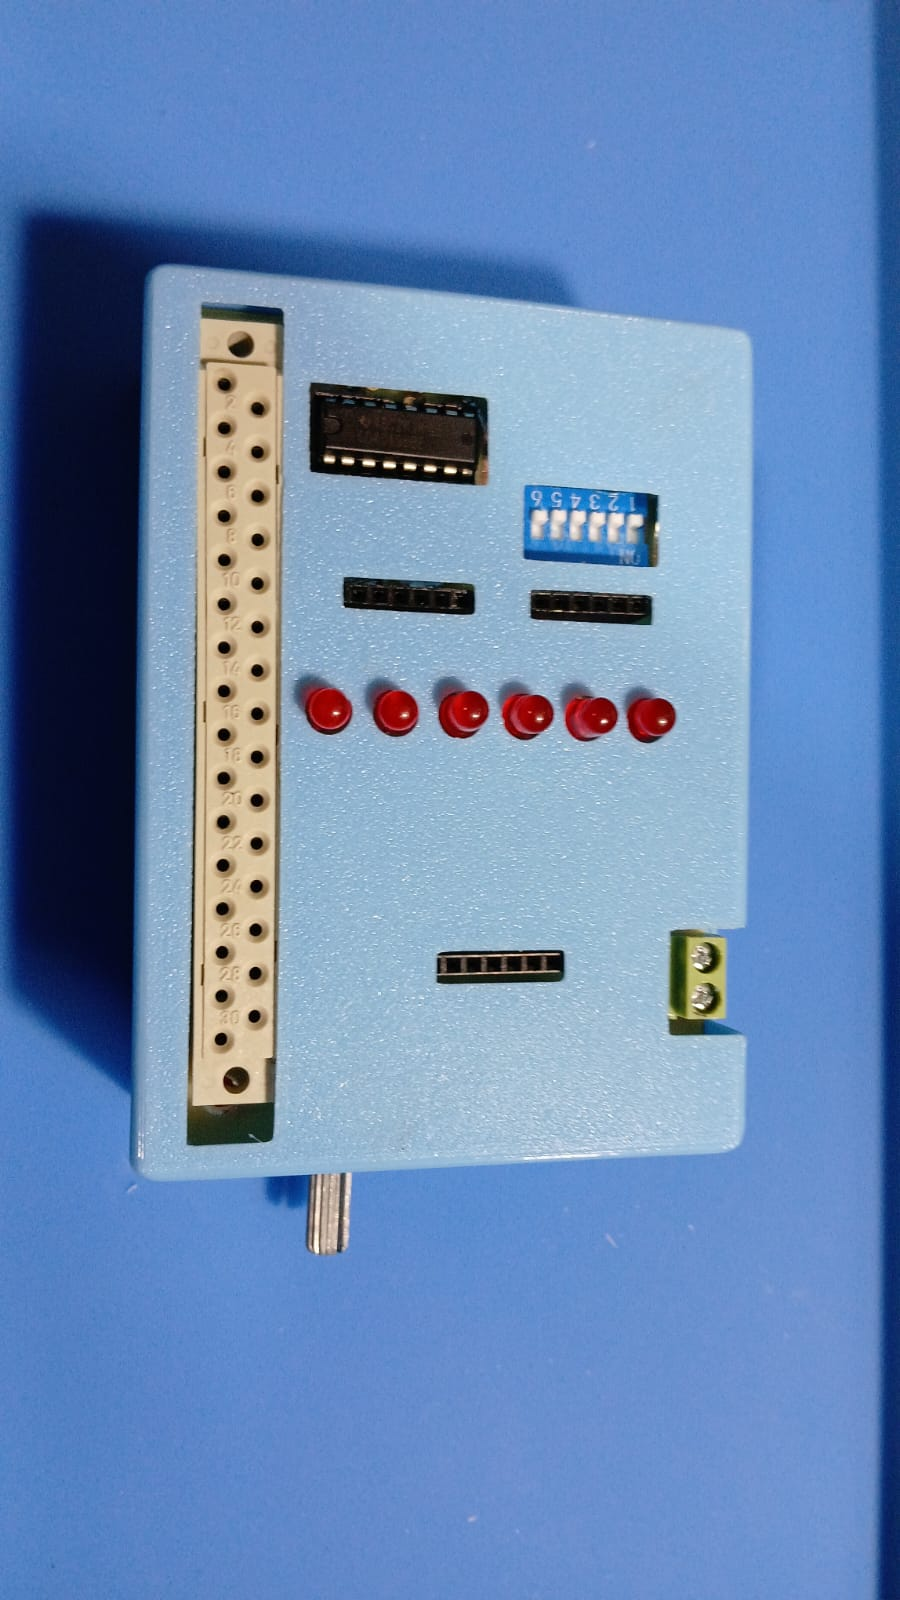
\includegraphics[width=0.4\textwidth,angle=90]{final.jpeg} 
	\caption{Mini-Lab terminado.}
\end{figure}

\section*{Dificultades encontradas}
\addcontentsline{toc}{section}{Dificultades encontradas}

Problemas de falso contacto y cortocircuitos por la distancias en entre las pistas de cobre.


\section*{Conclusiones}
\addcontentsline{toc}{section}{Conclusiones}
El Mini-Lab construido cumple satisfactoriamente con los requisitos de la cátedra, resultando en una plataforma confiable, portátil y funcional para la experimentación en Técnicas Digitales I. El proceso de diseño y fabricación fue fundamental para afianzar conocimientos prácticos en simulación, ruteado de PCB, técnicas de soldadura y prototipado de pcb.


\section*{Anexo: Acceso Digital}
\addcontentsline{toc}{section}{Anexo: Acceso Digital}

Para facilitar la visualización del informe original y los archivos de diseño en el repositorio de GitHub, se adjunta el siguiente código de acceso:




\begin{figure}[H]
	\centering
	\qrcode[height=4cm]{https://github.com/Enig17/Minilab/blob/e52050b55164b2b7c851671032eec42dd64bc2e2/Informe/TP0.pdf}
	\caption{Código QR para acceso al informe en línea.}
		\small \textbf{Link:} \url{https://github.com/Enig17/Minilab/blob/main/Informe/TP0.pdf}
\end{figure}
	


	
\end{document}